\documentclass[conference]{SIGCOMM}

\let\labelindent\relax
\usepackage{enumitem}\setlist{nolistsep}

\usepackage{color}
\newcommand{\todoh}[1]{{\color{red} \{TODO (from Harshad): #1 \}}}
\newcommand{\todod}[1]{{\color{blue} \{TODO (from Dayoon): #1 \}}}

\usepackage{url}
\usepackage{graphicx}
\newcommand\blfootnote[1]{%
  \begingroup
  \renewcommand\thefootnote{}\footnote{#1}%
  \addtocounter{footnote}{-1}%
  \endgroup
}

\usepackage{listings,textcomp,color}
\lstset{language=Python,upquote=true,
  basicstyle=\scriptsize,commentstyle=\textit,stringstyle=\upshape,
  numbers=left,numberstyle=\scriptsize,stepnumber=1,numbersep=5pt,
  backgroundcolor=\color{white},frame=single,tabsize=2,
  showspaces=false,showstringspaces=false,showtabs=false,
  breaklines=true,breakatwhitespace=true,escapeinside=||
}

%
\def\sharedaffiliation{%
\end{tabular}
\begin{tabular}{c}}
%

\usepackage{caption,subcaption} % Subfigures

\begin{document}

\title{Effect of Chunk Size on Router Caches for Video Based Workloads
    in Information-Centric Networks}

\numberofauthors{1}
\author{
  \alignauthor{Harshad Shirwadkar, Da-Yoon Chung} \\
  \email{harshad@cmu.edu, dayoonc@andrew.cmu.edu} \\
  \sharedaffiliation
  \affaddr{Carnegie Mellon University }   \\
  \affaddr{Pittsburgh, PA 15213. }
%%  Paper \#163: 12 Pages
}

\maketitle

\begin{abstract}
Caching in routers has been widely explored, with some models of networking such
as Content Centric Networking already providing implementations of such
functionality. While the effects of many different parameters of caching has
been quantified and studied, one aspect has largely been ignored: the chunk size
of the content being cached. Our work attempts to explore this single aspect of
caching and its effect on previously established metrics on both user experience
and server performance.
\end{abstract}

% A category with the (minimum) three required fields
\category{C.2}{Computer-Communication Networks}{Miscellaneous}
\category{C.4}{Performance of Systems}{Measurement Techniques}

\terms{Measurement, Performance, Experimentation}

\keywords{ICN, CCN, NDN, Video} % NOT required for Proceedings

\section{Introduction} \label{sec:Intro}

The idea of introducing caching to network routers is not a novel one. As the
type of network traffic shifted from mostly host-to-host connections to content
based traffic, it became clear that caching could provide savings as popular
content was requested frequently by many different clients. Some recent work by
Sun et al focuses on streaming video as a major source of traffic in modern
networks \cite{2}, and as the size of these videos and available user bandwidth both
increase today, we will see more and more redundant data make its way across
the internet. By introducing network caches, it has been shown that a
significant reduction in network traffic is achievable. However, while these
publications take into account many different aspects of router caches such as
cache placement and size, they sidestep a potentially important parameter: the
size of the individual chunks themselves. 

In this project, we explore the effects of chunk size on a number of previously
established metrics for both user quality of experience and server performance.
More specifically, we measure join time, buffering ratio, pending interest table
size, server load reduction, and total video view time. Using the ndnSIM module 
for the NS-3 network simulator, we designed a client and server application to quantify
these metrics. We run our experiments on a small, straightforward topology which
while not accurately representative of the real world, demonstrates the type of
results we would expect in practice. 


\section{Background} \label{sec:background}
In order to better introduce the question we are trying to answer, we will talk
about our work in relation to two previously published papers. The first is
called ``Developing a Predictive Model of Quality of Experience for Internet
Video'' \cite{1}. This paper redefines the metrics used to predict the quality of
experience that a user experiences depending on a number of measurements of
video streaming. Although not directly related to caching, we used this work to
determine which metrics we would try to measure to make sure our results
translated to effects on the user.

The second paper is called ``Trace-Driven Analysis of ICN Caching Algorithms on
Video-on-Demand Workloads'' \cite{2}. This work is actually where we got the idea for
our own project. We chose to explore one of the few aspects of caching that the
paper did not take into account.

\section{Approach} \label{sec:approach}
We discussed two different possibilities for running our experiments. The first
option we considered was using real hardware to run the client, router, and
server nodes for our experiments. The advantage of this approach is that it
would be as close to a real, albeit very small, network in the real world. The
obvious downside to this approach is the difficulty in setting up experiments,
especially in implementing caching in commercial routers if we wanted to go all
the way with this approach. There are testbeds like emulab which we had
previous experience using that allow experiments to easily define physical nodes
and links in a network, but these do not provide any customization capabilities
for the routers involved in the links. We quickly decided not to pursue this
route.

The second approach, which was ultimately better suited to our purposes, is a
simulation and trace-driven approach, similar to [2]. Using simulation software
allowed us to run many different configurations of experiments on individual
machines, and to predefine workloads that we could keep constant across runs.
Because we did not have to worry about acquiring and  transferring real files in
our experiments, we could instead just simulate their effects on the network.
This approach was easier than the former, while still being able to produce
valid results.

\subsection{ndnSIM} \label{sec:ndnSIM}
ndnSIM is a NS-3 based simulator for Named Data Networking (NDN), a networking
model very similar to Content Centric Networking (CCN). It allows users to set
up custom topologies, and define the behavior of individual nodes in the network
using custom applications. In terms of our intended use of simulating the
transfer of chunks between servers and clients in a network, ndnSIM is perfect
because it already abstracts these content chunks into data and interests.
Another big draw of ndnSIM is that it already has an implementation of a cache
in the form of a Content Store structure. These Content Store objects are more
general than the router caches we want to test, because they can be placed on
any nodes in the network (not just routers). They are minimally configurable,
allowing users to set the eviction policy and the max size in terms of packets. 

\section{Experimentation} \label{sec:experimentation}

\subsection{Topology} \label{sec:topology}

The most simple example of a topology involving a client, router, and server
would be a three node setup with links between the client and router and router
and server. However, we would only expect to router cache hits if the same video
was requested multiple times, which while not unlikely due to our
zipf-distribution of video popularity, is a poor representation of reality, and
is also very boring.

We therefore ran our experiments on a more complex topology involving five
clients linked to a single router, which in turn is linked to a server.

\begin{figure}[h]
    \begin{center}
        \begin{tabular}{c}
            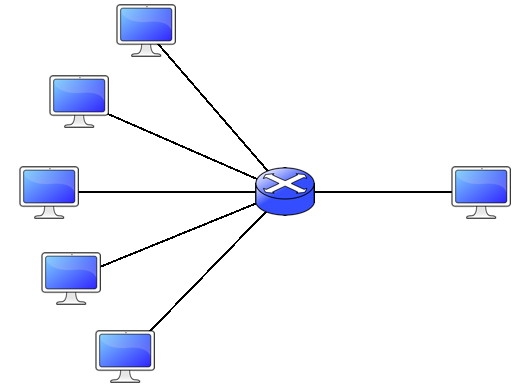
\includegraphics[width=0.45\textwidth]{fig/topology.png} \\
        \end{tabular}
        \caption{Topology for the experiments}
        \label{fig:topology}
    \end{center}
\end{figure}

The bandwidth of the links between the nodes is 10  mbps with
10 ms of latency. With our workload, we do not  see enough traffic for
congestion to affect our results.



\subsection{Client Application} \label{sec:client}

In order to run our experiments, we had to define a custom client application.
Our client application is simple. First, we pre-generated trace files for each
client, indicating which videos the each client would request, in what order,
and to what ending duration. As we previously mentioned, the videos are chosen
from a zipf distribution of popularity. Because we use these traces, each
experiment we run for different chunk sizes requests the same videos. This
ensures that our results will not have any discrepancies due to random
differences in viewing, but on the downside, our results might not be
representative of the average behavior. We made this compromise in the interest
of time, but ideally, we could have run many randomized experiments multiple
times and found an average.
In order to better replicate real-world video streaming applications, we define
a buffer which is 0.1 times the length of the video. Instead of beginning the
simulating watching of the video once the first chunk is received, which we had
done originally, we begin the watching of the video once the buffer is full for
the first time. Once the video has begun to be watched, we track the current
play time of the video and the amount of data fetched separately. The buffer
slides along with the current play time such that the client tries to always
have the next 10\% of the chunks of the video pre loaded. The client would be
considered to be in a buffering state if the current play time catches up to the
last chunk fetched in the buffer.

Once a client reads in a video to watch from its corresponding trace file, it
begins requesting chunks of the video to the server by sending interests. The
clients do not specify the size of the chunk in the requests; this is defined in
the server application. Instead, the client determines the size of the chunk by
checking the size of the data received. Once data is received, the client
updates the buffer, checks if its buffer is full, and requests another chunk if
it is not. If it is full, the client waits until another chunk's worth of play
time has passed, and then requests another chunk.

\subsection{Server Application} \label{sec:server}

The server waits for an interest to be received, and when it does, it returns of
chunk to the client, which is a data buffer of the chunk size being measured for
that experiment. The content of the chunk is currently not checked by either the
server or the client, so there is no content verification in place. This is
really the extent of what the server does.

\subsection{Router} \label{sec:router}

The router is not something we programmed, but we did configure it. As was
mentioned before, the size of the router is defined in terms of the number of
packets, rather than an absolute size. Therefore, we set the size to be equal to
7 MB, a value small enough that on average, an entire video could not exist in
the cache at one time.

We also used the router to observe the pending interests table, a data structure
which tracks which interests were received but not yet served by the router.
This is unique to these content centric network models.

\subsection{MTU} \label{sec:mtu}

ndnSIM has a default MTU value of 1500 bytes, which is in line with the maximum
packet size allowed by ethernet. Unfortunately, this means that if we experiment
with chunks larger than this value, ndnSIM automatically breaks them up into
multiple packets, which are then individually cached by the content store. If we
then want to evict a logical chunk from the cache, we have to modify ndnSIM to
ensure that all of the chunks corresponding to the chunk is evicted. 

In order to circumvent this complication, we configured ndnSIM to have an MTU
much larger than any of the chunk sizes we experimented with. Although this does
not model the real world perfectly, we felt this was an acceptable compromise
because it would allow us to trust the cache to behave as we expected.

\subsection{Batching} \label{sec:batching}

In some initial runs of our experiment, we did not implement any batching of
requests by the client. Individual chunks were requested in order, one after the
other. Unsurprisingly, certain metrics we chose like start-up time suffered
miserably as RTT for the packets (40 ms, with our particular topology) consumed
the vast majority of the time before the initial buffer filled and the video
started being watched.

For later experiments, we implemented batching on the client. Instead of
individual interests, the client computes which chunks in the buffer are not yet
fetched, and sends individual interests for those chunks all at once. Once it
receives all of the data for this batch of requests, it repeats the process. The
effects of this are quantified in the results section.

\section{Evaluation} \label{sec:eval}

\subsection{Metrics Evaluated} \label{sec:metrics}

Join Time: This metric was used in the QoE paper as a measure of user
experience. It refers to the time it takes for the video to start playing after
it has been requested. Because we also used a video-based workload, we believed
this was still a very relevant metric.

Buffering Ratio: This metric was also used in the QoE paper. This is the ratio
between the  time that the user spends waiting for the video to buffer and the
total time to finish watching the video. We felt this would also be an
interesting metric, because we expected it to vary inversely with chunk size, as
it would take longer for increments of the video to be buffered. However, it is
possible that our buffer size is large enough that we prefetch enough chunks
that this is not the case.

Pending Interest Table Size: This structure is import to us because we expected
the number of pending interests to vary inversely with the chunk size. With
smaller chunks, chunk request are made more frequently because the buffer
empties in smaller increments, so more requests should pile up on the router
node.

Server Load Reduction: This is fraction of requests that was served by the cache
rather than the server. This is a standard way to measure the benefits to the
server due to caching.

\subsection{Chunk Size} \label{sec:chunksize}

We ran experiments for the following chunk sizes (in bytes): 128, 256, 512,
1024, 1940, 4096, 6144, 8192. 1940 is an odd value because it is not 2048 as
would be expected given the other values. We had to use value because for reason
we could not identify, the data could not be received by the clients for any
chunk sizes between roughly 2000 to 3000. The server would receive the
interests, but the experiments would stop at that point. There were no other
error messages or information we could use to debug, so in the interest of time,
we used a value close to 2048 just to have a datapoint in the range of values.


\subsection{Experiments without batching} \label{sec:nobatch}

Not batching has the most extreme effect on the join time metric. For 128 byte
chunks, we see the join time is about 30 seconds, which is longer than the
length of most videos themselves. To deduce why this is the case, we can do some
simple calculations. Given we defined a buffering window of 10\% of the total
video size, for a video of size 10 MB, the client downloads 1 MB of the video
before starting the video. This is equal to $1 * 1024 * 1024 / 128 = 8192$
individual requests. The $RTT$ of each request is $4 * 10 = 40$ ms because
each link has $10$ ms latency. Therefore, just the time the chunks spend in
transit is equal to $8192 * 40 = 327680$ milliseconds, or 328 seconds.

With larger chunk sizes, we see the linear decrease in join time as we would
expect.



\section{Related Work} \label{sec:related}

\section{Future Work} \label{sec:futurework}




\section{Conclusion} \label{sec:conclusion}

In this work, we examined the effect of different chunk lengths on
Video QOE metrics as well as cache and server performance. Many
researchers in this area assume a particular chunk size and base their
research on that. Our simulations clearly suggested that it is
important to take into account the size of chunks in any upcoming
research in information centric networks. Our key findings about chunk
sizes are: 1) Higher chunk sizes tend to have lower PIT overhead and
lower cache performance win 2) Lower chunk sizes, on the other hand,
have lower PIT overhead and lower cache performance.
If a network administrator values server resources over user quality of
experience, he or she could use smaller chunk sizes. However, if they value the
performance of the network even at the expense of lower server saving, they
should use a bigger chunk size.

Based on these
findings, we believe that future research in this space should definitely take
into account the performance of different workloads for various chunk sizes.

\bibliographystyle{abbrv}
\bibliography{refs}

\end{document}
